\documentclass[a4paper,cs4size]{BHCexam}
%\documentclass[a4paper,cs4size,answers]{BHCexam}

\usepackage{multicol} % 分栏
\usepackage{hyperref}
\pagestyle{fancy}
\fancyfoot[C]{\kaishu \small 第 \thepage 页 共 \pageref{lastpage} 页}
%\fancyhead[L]{\includegraphics[width=2cm]{qrcode.png}}
\title{压强习题课2}
%\subtitle{数学文科试卷}
%\notice{满分150分, 120分钟完成, \\	允许使用计算器,答案一律写在答题纸上.}
%\author{Gavin Chen}
%\date{\today}

\begin{document}
\maketitle
\begin{groups}
    \group{}{帕斯卡定律}
    斯卡定律:加在密闭液体上的压强能够大小不变地由液体向各个方向传递。实验表明,帕斯卡定律对气体也是适用的。
    注意,是增值被瞬间传递。

    动画:\href{https://www.bilibili.com/video/BV1EA411M7Zu/?spm_id_from=333.337.search-card.all.click&vd_source=2329e0d9ebf298ab4960a6d3a7eecf56}{Go to Bilibili}

    应用:液压机,千斤顶

    \zihao{-4}
    \begin{questions}[]

        \question[5] 如图所示,密闭容器内盛水,有一个力$F$压在横截面积为$S$的活塞上,则传递到$A$、$B$点的压强为(\quad\quad\quad)。
        \fourchoices{$p_A=p_B$}
        {$p_A<p_B$}
        {$p_A>p_B$}
        {无法判断}
        \begin{figure}[htb]
            \flushright
            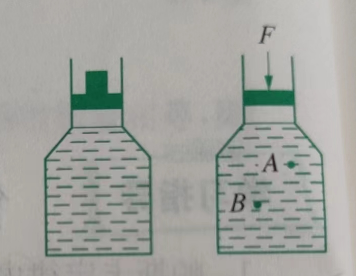
\includegraphics [scale=0.4,trim=0 0 0 0]{./image/physics_pressure2_1.png}
            % \caption{图名}
            \label{fig:fig_pressure2_1}
        \end{figure}
        \vspace{1cm}

        \question[5] 如图所示,甲、乙两个完全相同的薄壁圆柱形容器置于水平桌面上,两容器底部用一根细管相连,
        开始时,阀门$K$关闭。容器底面积均为$2\times 10^{-2}m^2$,甲中盛有深度为$0.2m$的水,乙中放一底面积为$1\times 10^{-2}m^2$,高为$0.2m$的
        圆柱形木块。
        \begin{subquestions}
            \subquestion 求甲中水对容器底部的压强$p_{\text{水}}$。
            \subquestion 若甲中水对容器底部的压强是乙中木块对乙底部压强的$2$倍,求木块的密度$\rho_{\text{木}}$。
            \subquestion 打开阀门,直到水不再流动,求此过程进入乙容器中水的质量$\Delta m_{\text{水}}$。
        \end{subquestions}
        \begin{figure}[htb]
            \flushright
            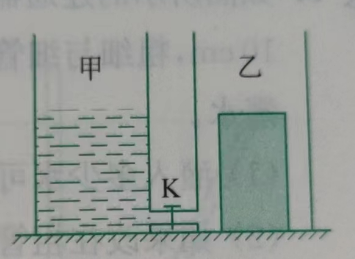
\includegraphics [scale=0.4,trim=0 0 0 0]{./image/physics_pressure2_2.png}
            % \caption{图名}
            \label{fig:fig_pressure2_2}
        \end{figure}
        \vspace{6cm}

        \question[5] 如图所示的连通器,粗管横截面积为$16cm^2$,其半径是细管半径的$2$倍,横管长$10cm$,
        粗细与细管一样。先把$0.24L$水银注入连通器内,然后在细管一端灌水。
        \begin{subquestions}
            \subquestion 灌入多少水可以灌满?
            \subquestion 如果改在粗管一端灌水,则需多少毫升水可以把粗管灌满?
        \end{subquestions}
        \begin{figure}[htb]
            \flushright
            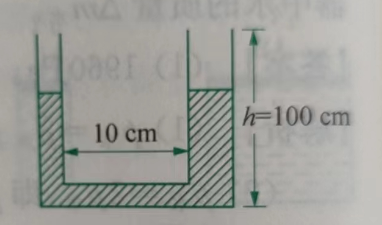
\includegraphics [scale=0.4,trim=0 0 0 0]{./image/physics_pressure2_3.png}
            % \caption{图名}
            \label{fig:fig_pressure2_3}
        \end{figure}
        \vspace{6.5cm}

        \question[5] 两端开口的玻璃管,一端盖有一块轻塑料片,塑料片浸入水下$10cm$处,从管口缓慢加水,
        当加入\underline{\quad\quad\quad\quad}$cm$高的水时,塑料片恰好下落;如果改为加入酒精,当加入
        \underline{\quad\quad\quad\quad}$cm$高的酒精时,塑料片恰好下落。
        \begin{figure}[htb]
            \flushright
            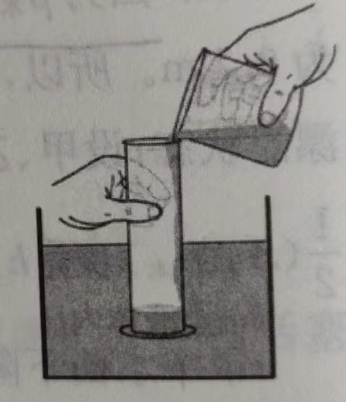
\includegraphics [scale=0.4,trim=0 0 0 0]{./image/physics_pressure2_4.png}
            % \caption{图名}
            \label{fig:fig_pressure2_4}
        \end{figure}
        \vspace{1.5cm}

        \question[5] 如图所示,水平放置的一根玻璃管和几个竖直放置的$U$形管内都有一段水银,
        封闭端里都有一定质量的气体,图A中的水银柱长度和图$B$、$C$、$D$中U形管两臂内水银柱高度差均为$h=10cm$,
        这四个管中气体压强最小的是(\quad\quad\quad)。
        \begin{figure}[htb]
            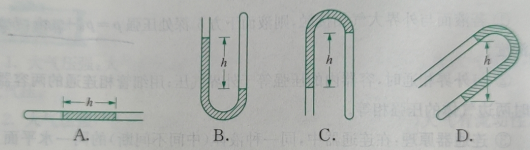
\includegraphics [scale=0.8,trim=0 0 0 0]{./image/physics_pressure2_5.png}
            % \caption{图名}
            \label{fig:fig_pressure2_5}
        \end{figure}
        \vspace{0.5cm}

        \question[5] 如图所示,活塞质量为$m$,缸套质量为$M$,通过弹簧吊在天花板上,
        气缸内封住一定质量的空气,且缸套与活塞间无摩擦,活塞截面积为$S$,大气压强为$p_0$,则(\quad\quad\quad)。
        \fourchoices{内外空气对缸套的作用力为$(M+m)g$}
        {内外空气对活塞的作用力为$mg$}
        {气缸内空气的压强为$p_0-\frac{Mg}{S}$}
        {气缸内空气的压强为$p_0+\frac{Mg}{S}$}
        \begin{figure}[htb]
            \flushright
            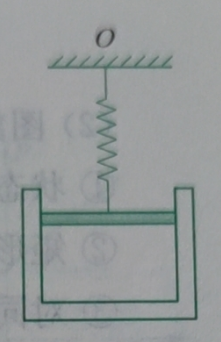
\includegraphics [scale=0.4,trim=0 0 0 0]{./image/physics_pressure2_6.png}
            % \caption{图名}
            \label{fig:fig_pressure2_6}
        \end{figure}
        \vspace{0.5cm}

        \question[5] 如图所示,一端封闭的玻璃管中有一些空气和一段水银柱,将它倒立在水银槽中,上端与弹簧秤相连,
        弹簧秤的挂钩挂在天花板上,则弹簧秤的示数为(\quad\quad\quad)。
        \fourchoices{玻璃管的重力和弹簧秤的重力之和}
        {玻璃管的重力和露出液面的那段水银柱的重力之和}
        {大气向上的压力减去玻璃管的重力}
        {玻璃管、弹簧秤和露出液面的那段水银柱的三者重力之和}
        \begin{figure}[htb]
            \flushright
            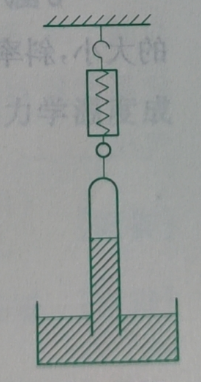
\includegraphics [scale=0.4,trim=0 0 0 0]{./image/physics_pressure2_7.png}
            % \caption{图名}
            \label{fig:fig_pressure2_7}
        \end{figure}
        \vspace{0.5cm}

        \question[5] 已知水银柱长$h=10cm$,大气压强$p_0=76cmHg$,分别求图中被水银封闭在容器$1,2,3$内的气体压强。
        $p_1=\underline{\quad\quad\quad}cmHg, p_2=\underline{\quad\quad\quad}cmHg, p_3=\underline{\quad\quad\quad}cmHg$
        \begin{figure}[htb]
            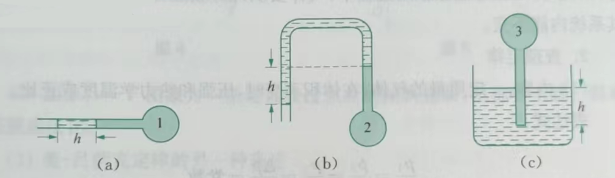
\includegraphics [scale=0.8,trim=0 0 0 0]{./image/physics_pressure2_8.png}
            % \caption{图名}
            \label{fig:fig_pressure2_8}
        \end{figure}
    \end{questions}





\end{groups}


\label{lastpage}
\end{document}
